\documentclass[a4paper]{article}
\usepackage[utf8]{inputenc}
\usepackage{amsmath, amssymb}
\usepackage{gensymb}
\usepackage{cancel}
\usepackage[nodayofweek]{datetime}

\usepackage{tikz}
\usepackage{tkz-euclide}
\usetikzlibrary{decorations.pathreplacing}

\usetikzlibrary{math}
\tikzmath{
	\rt = sqrt(3);
}
\tikzset{/tkzmkangle/mark=none}

% Set size of text area with total parameter
\usepackage[a4paper, total={135mm, 255mm}]{geometry}

\title{Circles in an Equilateral Triangle}
\author{Dyson}
\date{\today}

\begin{document}

\maketitle

% Set paragraph spacing here to avoid messing with title
\setlength{\parindent}{0em}
\setlength{\parskip}{1em}

This question places two circles and an equilateral triangle in a larger equilateral triangle and asks for the fraction of shaded area.

\vspace*{0.5em}
\hspace{\fill}
\begin{tikzpicture}[scale=1.5]
% C         B
%     F G
%      H
%   E     D
%
%      A
\coordinate (C) at ({-1-\rt},{3+\rt});
\coordinate (B) at ({1+\rt},{3+\rt});
\coordinate (A) at (0,0);
\coordinate (E) at ({(-3-\rt)/3},{1+\rt});
\coordinate (D) at ({(3+\rt)/3},{1+\rt});
\coordinate (F) at (-1,{2+\rt});
\coordinate (G) at (1,{2+\rt});
\coordinate (H) at (0,2);

\draw (A) -- (B) -- (C) -- cycle;
\draw[fill=gray!30] (A) -- (D) -- (E) -- cycle;
\draw (F) circle[radius=1];
\draw (G) circle[radius=1];
\end{tikzpicture}
\hspace{\fill}
\vspace*{0.5em}

We can start by trying to find how the two circles touch. We can imagine hexagonal circle packing and see that if we connect the centres of 3 adjacent circles, it forms an equilateral triangle.

\vspace*{0.5em}
\hspace{\fill}
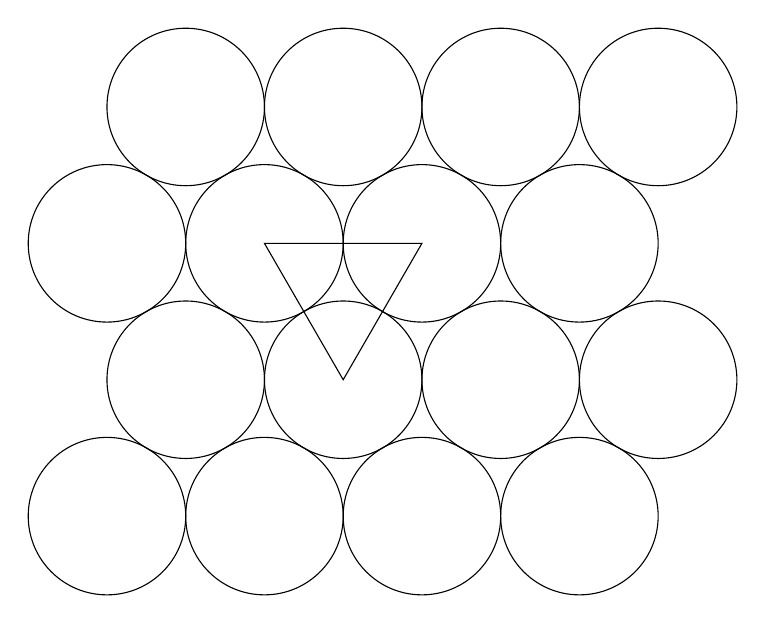
\begin{tikzpicture}
\draw (0,0) circle[radius=1];
\draw (2,0) circle[radius=1];
\draw (4,0) circle[radius=1];
\draw (6,0) circle[radius=1];

\draw (1,{sqrt(3)}) circle[radius=1];
\draw (3,{sqrt(3)}) circle[radius=1];
\draw (5,{sqrt(3)}) circle[radius=1];
\draw (7,{sqrt(3)}) circle[radius=1];

\draw (0,{2*sqrt(3)}) circle[radius=1];
\draw (2,{2*sqrt(3)}) circle[radius=1];
\draw (4,{2*sqrt(3)}) circle[radius=1];
\draw (6,{2*sqrt(3)}) circle[radius=1];

\draw (1,{3*sqrt(3)}) circle[radius=1];
\draw (3,{3*sqrt(3)}) circle[radius=1];
\draw (5,{3*sqrt(3)}) circle[radius=1];
\draw (7,{3*sqrt(3)}) circle[radius=1];

\draw (3,{sqrt(3)}) -- (2,{2*sqrt(3)}) -- (4,{2*sqrt(3)}) -- cycle;
\end{tikzpicture}
\hspace{\fill}
\vspace*{0.5em}

We can then isolate these three circles, wrap this construction in another equilateral triangle, and consider how the two triangles are related.

\vspace*{0.5em}
\hspace{\fill}
\begin{tikzpicture}[scale=1.5]
\draw (F) circle[radius=1];
\draw (G) circle[radius=1];
\draw (H) circle[radius=1];
\draw (F) -- (G) -- (H) -- cycle;
\draw (A) -- (B) -- (C) -- cycle;
\end{tikzpicture}
\hspace{\fill}
\vspace*{0.5em}

We can draw the radii of the circles, perpendicular to the triangles and define a value of 1 for these radii.

\vspace*{0.5em}
\hspace{\fill}
\begin{tikzpicture}[scale=1.5]
\draw (F) circle[radius=1];
\draw (G) circle[radius=1];
\draw (H) circle[radius=1];
\draw (F) -- (G) -- (0,2) -- cycle;
\draw (A) -- (B) -- (C) -- cycle;

% These coords form line perpendicular to the triangles with the F, G, and H
%   a     b
%  f       c
%
%    e   d
\coordinate (a) at (-1,{3+\rt});
\coordinate (b) at (1,{3+\rt});
\coordinate (c) at ({1+sin(60)},{2+\rt-sin(30)});
\coordinate (d) at ({sin(60)},{2-sin(30)});
\coordinate (e) at ({-sin(60)},{2-sin(30)});
\coordinate (f) at ({-1-sin(60)},{2+\rt-sin(30)});

\draw (F) -- node[right] {1} (a);
\draw (G) -- node[left] {1} (b);
\draw (G) -- node[below] {1} (c);
\draw (H) -- node[above] {1} (d);
\draw (H) -- node[above] {1} (e);
\draw (F) -- node[below] {1} (f);

\tkzMarkRightAngle[size=0.15](a,F,G);
\tkzMarkRightAngle[size=0.15](F,G,b);
\tkzMarkRightAngle[size=0.15](c,G,H);
\tkzMarkRightAngle[size=0.15](G,H,d);
\tkzMarkRightAngle[size=0.15](e,H,F);
\tkzMarkRightAngle[size=0.15](H,F,f);
\end{tikzpicture}
\hspace{\fill}
\vspace*{0.5em}

Because the length of the small equilateral triangle is made of two radii, we know that it's 2.

This 2 extends to give us part of the length of the big triangle, and then we can zoom in on one of the kites in the corners to find the rest of the length.

\vspace*{0.5em}
\hspace{\fill}
\begin{tikzpicture}[scale=1.5]
\draw (G) -- node[below] {1} (c) -- node[right] {$x$} (B) -- node[above] {$x$} (b) -- node[left] {1} cycle;
\draw (G) -- (0.5,{2+\rt-sin(60)});
\draw (G) -- (0,{2+\rt});

\tkzMarkRightAngle[size=0.15](F,G,b);
\tkzMarkRightAngle[size=0.15](c,G,H);
\tkzMarkRightAngle[size=0.15](B,b,G);
\tkzMarkRightAngle[size=0.15](B,c,G);

\tkzMarkAngle[size=0.3](F,G,H);
\tkzLabelAngle[pos=0.5](F,G,H){$60\degree$};
\tkzMarkAngle[size=0.3](c,G,b);
\tkzLabelAngle[pos=0.6](c,G,b){$120\degree$};
\tkzMarkAngle[size=0.3](b,B,c);
\tkzLabelAngle[pos=0.6](b,B,c){$60\degree$};
\end{tikzpicture}
\hspace{\fill}
\vspace*{0.5em}

We can use the exterior angles of $90\degree$, $90\degree$, and $60\degree$ to find the interior angle to be $120\degree$. With the knowledge of the right angles of the kite, we can find the opposite angle to be $60\degree$.

We can divide the kite into triangles and use the sine rule to find the missing length $x$.

\vspace*{0.5em}
\hspace{\fill}
\begin{tikzpicture}[scale=1.5]
\draw (G) -- node[below] {1} (c) -- node[right] {$x$} (B) -- node[above] {$x$} (b) -- node[left] {1} cycle;

\tkzMarkRightAngle[size=0.15](B,b,G);
\tkzMarkRightAngle[size=0.15](B,c,G);

\tkzMarkAngle[size=0.3](c,G,B);
\tkzLabelAngle[pos=0.6](c,G,B){$60\degree$};
\tkzMarkAngle[size=0.4](G,B,c);
\tkzLabelAngle[pos=0.7](G,B,c){$30\degree$};

\draw[dotted] (G) -- (B);
\end{tikzpicture}
\hspace{\fill}
\vspace*{0.5em}

We know that
\begin{gather*}
\frac{x}{\sin 60\degree} = \frac{1}{\sin 30\degree}\\[0.5em]
\therefore x = \frac{\sin 60\degree}{\sin 30\degree} = \sqrt{3}
\end{gather*}

Since $x = \sqrt{3}$, we can now find the length of the big triangle to be $2 + 2\sqrt{3}$.

We're now going to plot the diagram in Cartesian coordinates. That's what I need to do to create these diagrams with TikZ, so that's the method I used.

To determine the coordinates of the corner of the larger triangle, we can draw a right triangle.

\vspace*{0.5em}
\hspace{\fill}
\begin{tikzpicture}[scale=1.5]
\coordinate (cc) at ({1+\rt},0);
\draw (A) -- node[below] {$x$} (cc) -- node[right] {$y$} (B) -- node[left] {$2+2\sqrt{3}$} cycle;

\tkzMarkRightAngle(B,cc,A);
\tkzMarkAngle(A,B,cc);
\tkzLabelAngle[pos=1.3](A,B,cc){$30\degree$};
\tkzMarkAngle(cc,A,B);
\tkzLabelAngle[pos=1.3](cc,A,B){$60\degree$};
\end{tikzpicture}
\hspace{\fill}
\vspace*{0.5em}

By the sine rule again, we can see that
\begin{gather*}
\frac{x}{\sin 30\degree} = \frac{y}{\sin 60\degree} = \frac{2 + 2\sqrt{3}}{\sin 90\degree} = 2 + 2\sqrt{3}\\[0.5em]
\therefore x = (2 + 2\sqrt{3}) \sin 30\degree = 1 + \sqrt{3}\\[0.5em]
y = (2 + 2\sqrt{3}) \sin 60\degree = 3 + \sqrt{3}
\end{gather*}

We now have the height of the larger triangle to be $3 + \sqrt{3}$. This means the height of the smaller triangle is the height of the bigger triangle minus twice the radius of the circles. Since the radius is 1, the height of the smaller triangle is $3 + \sqrt{3} - 2 = 1 + \sqrt{3}$.

We can then draw another right triangle and use the sine rule again to find the coordinates of the top corner of the smaller triangle.

\vspace*{0.5em}
\hspace{\fill}
\begin{tikzpicture}[scale=1.5]
\coordinate (dd) at ({(3+sqrt(3))/3},0);
\draw (A) -- node[below] {$x$} (dd) -- node[right] {$1 + \sqrt{3}$} (D) -- node[left] {$\ell$} cycle;

\tkzMarkRightAngle(D,dd,A);
\tkzMarkAngle[size=0.5](A,D,dd);
\tkzLabelAngle[pos=0.8](A,D,dd){$30\degree$};
\tkzMarkAngle[size=0.5](dd,A,D);
\tkzLabelAngle[pos=0.8](dd,A,D){$60\degree$};
\end{tikzpicture}
\hspace{\fill}
\vspace*{0.5em}

We don't care about $\ell$, but we can find $x$ with the sine rule.
\begin{gather*}
\frac{x}{\sin 30\degree} = \frac{1 + \sqrt{3}}{\sin 60\degree}\\[0.5em]
\therefore x = \frac{(1 + \sqrt{3}) \sin 30\degree}{\sin 60\degree} = \frac{3 + \sqrt{3}}{3}
\end{gather*}

We now have everything we need to compute the areas of the triangles, and then we can compute the fraction of shaded area.

The area of the larger triangle is
\begin{gather*}
\frac{1}{2} \times b \times h\\[0.5em]
= \frac{1}{2} \times (2 \times (1 + \sqrt{3})) \times (3 + \sqrt{3})\\[0.5em]
= (1 + \sqrt{3})(3 + \sqrt{3})\\[0.5em]
= 6 + 4\sqrt{3}
\end{gather*}

The area of the smaller triangle is
\begin{gather*}
\frac{1}{2} \times b \times h\\[0.5em]
= \frac{1}{2} \times \left(2 \times \left(\frac{3 + 3\sqrt{3}}{3}\right)\right) \times (1 + \sqrt{3})\\[0.5em]
= \left(\frac{3 + 3\sqrt{3}}{3}\right)(1 + \sqrt{3})\\[0.5em]
= \frac{6 + 4\sqrt{3}}{3}
\end{gather*}

Therefore, the fraction of shaded area is $$\frac{\left(\frac{6 + 4\sqrt{3}}{3}\right)}{6 + 4\sqrt{3}} = \frac{1}{3}$$

\hspace{\fill}$\square$

\end{document}
